\section{Implementation and Optimization on GPU}
\label{sec:implementation}
In this section, we describe the implementation of bisection and twisted algorithm on a GPU.
%A GPU with CUDA architecture typically uses Single Program Multiple Threads (SPMT) model to execute its workload. 
%A GPU thread is the fundamental working unit of a parallel program and a GPU warp consists of 32 concurrent threads. 
%A GPU block is a group of threads sharing data via the shared memory, and the number of threads per block is typically a multiple of 32 and ranges from 256 to 1024. The number of threads per block determines the number of warps, which are assigned to GPU's cores by its internal scheduler.
%The goal of implementing our BT algorithm is to maximize the warp execution efficiency, which is defined as the average percentage of active threads in each executed warp to take full advantage of GPU resources.

%We implement our BT algorithm in two steps: 
%we design singular value kernels in the first step (Section \ref{sec_svalue}) and singular vector kernels in the second step (Section \ref{sec_svector}), and then map them onto the appropriate GPU components. We also leverage GPU-specific optimizations for handling huge matrix from big data applications.

\subsection{Singular Value Kernels}
\label{sec_svalue}
To obtain the singular values, we divide the whole interval calculated with Gershgorin circle theorem into several subintervals, which can be computed in parallel.
Each subinterval can then be assigned to one GPU block for calculation.
Because there is a limit on the maximum number of threads for each GPU block,
the number of singular values in a subinterval must not exceed that maximum number. Otherwise, the computation will have to be wrapped into two or more sequential phases to complete.
Therefore how to divide the interval is critical for the performance of
computing singular values. We consider two different partition
strategies as described below. 
\begin{figure}[hbpt]
\vspace{-0.3in}
\centering
  \subfigure[Equal Length Division]
  {
  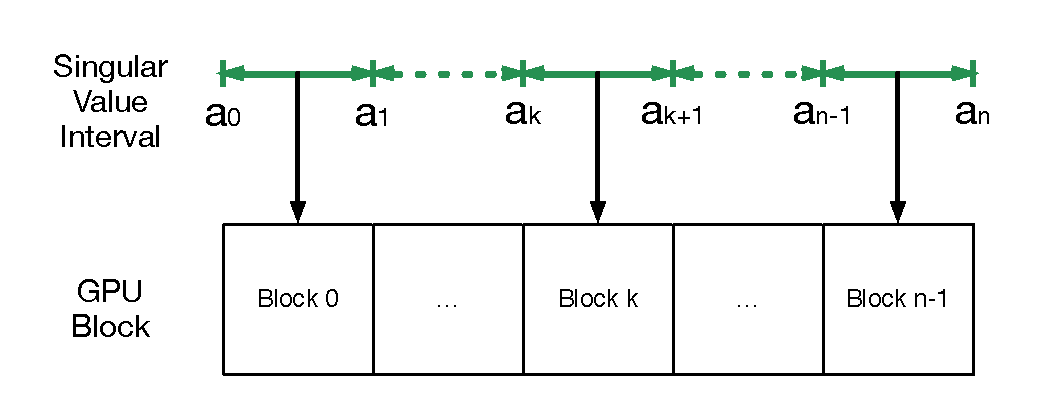
\includegraphics[width=0.45\textwidth]{length_interval}
  \label{fig:length_interval}
  }
  \subfigure[Equal Number Division]
  {
  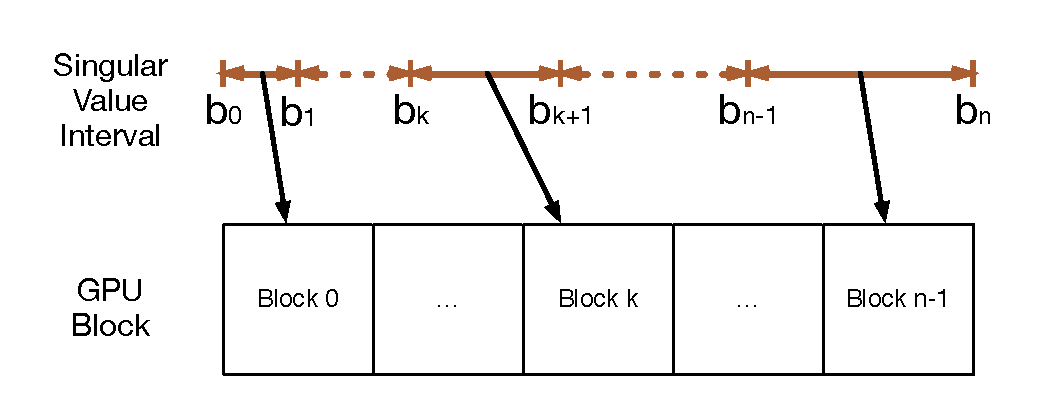
\includegraphics[width=0.45\textwidth]{number_interval}
  \label{fig:number_interval}
  }
  \vspace{-0.1in}
  \caption{Division Strategies for Partitioning Interval  $[a_0, a_n)$.}
\vspace{-0.3in}
\end{figure}

The first (na\"{\i}ve) strategy is to divide the interval into chunks of equal length as shown in Fig.\ref{fig:length_interval}.
The whole interval $[a_0, a_n)$ is divided into $n$ subintervals with
the same length (i.e. same number of matrix elements). However, each
such  subinterval might not contain the same number of singular values.
Mathematically, this strategy can be expressed as
% $a_{k+1}-a_k = a_{k}-a_{k-1}$ and $NegCount(b_{k+1})-NegCount(b_{k}) \ne NegCount(b_{k})-NegCount(b_{k-1})$.
%\begin{eqnarray}
$a_{k+1}-a_k = a_{k}-a_{k-1}$ %\hspace{2cm} 
%\end{eqnarray}
However,
%\begin{eqnarray}
$NegCount(a_{k+1})-NegCount(a_{k}) = NegCount(a_{k})-NegCount(a_{k-1})$
%\end{eqnarray}
is not necessarily true. We call this strategy as {\it equal length division}.

%\begin{algorithm}
%\small
\caption{Equal Length Subinterval Algorithm}
\label{alg:lengthsub}
\begin{algorithmic}[1]
\Procedure{$\mathbf{Length\_Divide}$}{$n, B, t, \tau$}
  \State Obtain singular value boundary $[l,u)$ of matrix $B$;
  \State Define the thread ID $i$, $i<t$;
  \State Obtain average step $s = (u-l) / t $;
  \State Lower bound $\alpha = l + i * s$;
%  \State Upper bound $\beta = max(l + (i+1) * s, \alpha)$;
  \State $n_{\alpha} = NegCount(\alpha)$;
%  \State $n_{\beta} = NegCount(\beta)$;
%  \State $\alpha = \min(\alpha,\beta)$;
%  \State $\beta = \max(\alpha, \beta)$;
%  \State $n_{\alpha} = \min(n_{\alpha},n_{\beta})$;
%  \State $n_{\beta} = \max(n_{\alpha}, n_{\beta})$;
%  \State Max scan to refine $\alpha, \beta, n_{\alpha}, n_{\beta}$
%  \State Call $Bisection(val, n, B, \alpha, \beta, n_{\alpha}, n_{\beta}, \tau)$
  \State save the division point $\alpha$ and $n_{\alpha}$
\EndProcedure
\end{algorithmic}
\end{algorithm}

%The parallel algorithm of length division working in GPU threads is shown in Algorithm \ref{alg:lengthsub}.

Such ``equal length division'' strategy has issues in load balancing on 
parallel computing resources, as the number of singular values in each
subinterval is not uniform. As a result,
the SVD workload cannot be easily balanced on GPU's processing cores to achieve a satisfactory speedup because the optimal number of subintervals is dependent on multiple factors, such as the maximum number of threads, the number of threads in a GPU warp, and the size of matrix.
%The maximum number of threads per block determines the minimum number
%of blocks should be allocated. 
The maximum number of threads per block determines the minimum number
of subintervals that are assigned to corresponding GPU blocks.
In addition, the number of threads in a GPU warp assigned to a subinterval affects the GPU utilization level.

We have conducted experiments to understand the trade-offs %of 
between subinterval length
and the GPU execution efficiency. Smaller subintervals will lead to a larger number of subintervals, which cause the GPU warp execution to be less efficient. 
For example, our experiments show that if $512$ subintervals are used, the efficiency of GPU warp execution ranges from only 12.38\% to 52.15\% when the matrix size increases from $1,000$ to $17,000$.
That is, only half of the threads in a warp work in parallel at most. This is because  (1)
 there are fewer singular values than the number of warps, leading the cores under-utilized; and 
(2) the warps are stalled due to memory accesses.

On the other hand, we can divide the whole interval into larger subintervals, making the total number of subintervals small. 
Then some of them may require much more processing capability
because these subintervals may contain more singular values than others.
In order to achieve a higher speedup, we could try to find the optimal number of subintervals, or the number of blocks, based on experimental results. 
%Our goal is to find the optimal number of subintervals, or the number of blocks, based on experimental results. Figure \ref{fig:length_block_num} shows the optimal number of blocks. As you can see that
%the performance has a 3.5 to 1.2 speedup compared to the a fixed subintervals.
%The warp execution efficiency improves to 31.40\%-78.45\%.
However, because of the uneven number of singular values within subintervals, the speedup for equal length division remains very limited, which motivates us to search for a better partition method.

Our novel strategy is to divide the whole interval by the number of singular values, as shown in Fig.\ref{fig:number_interval}. We call this approach {\it equal number division}. 
Specifically, we divide the interval $[b_0,b_n)$ into $n$ subintervals, each of which has the same number of singular values. 
However, the length of a subinterval is not necessarily equal to others.
The mathematical representation can be written as %$NegCount(b_{k+1})-NegCount(b_{k})=NegCount(b_{k})-NegCount(b_{k-1})$ but $b_{k+1}-b_k \ne b_{k}-b_{k-1}$
%\begin{eqnarray}
$NegCount(b_{k+1})-NegCount(b_{k}) = NegCount(b_{k})-NegCount(b_{k-1})$
%\end{eqnarray}
but $b_{k+1}-b_k = b_{k}-b_{k-1}$ does not hold anymore.
This equal number division significantly improves the load balancing on GPU cores, helping achieve a better speedup.

The convergence of bisection algorithm on a splitting point makes it possible to compute the number of singular values before actually computing
the values themselves. The splitting point can be easily found by applying several $NegCount$ functions on the interval. Specifically, we design a method to find the boundary points of such subintervals, as shown in Algorithm \ref{alg:numsub}.
%Line 2 is to obtain the whole interval of matrix $B$.
Lines 4-5 find the midpoint of interval and its corresponding $NegCount$.
Lines 6-15 make use of loop to find the split point of number division by bisection algorithm.
%Line 6-16 make use of loop to find the split point of number division by bisection algorithm.
\begin{algorithm}
%\small
\caption{Equal Number of Singular Value Subinterval Algorithm}
\label{alg:numsub}
\begin{algorithmic}[1]
\Procedure{$\mathbf{Number\_Divide}$}{$n, B, t, \tau$}
  \State Obtain singular value boundary $[l,u)$ of matrix $B$;
  \State Define the thread ID $i$, $i<t$;
  \Comment t is total threads
  \State $mid = inside(l, u, B)$;
  \State $n_m = NegCount(n, B, mid)$;
  \While {$n_m \ne (i+1)n/t$ and $mid-l > \tau$}
    \If {$n_m \ge (i+1)n/t$}
      \State $u=mid$;
      \State $n_u=n_m$;
    \Else
      \State $l=mid$;
      \State $n_l=n_m$;
    \EndIf
    \State $mid = inside(l, u, B)$;
    \State $n_m = NegCount(n, B, mid)$;
  \EndWhile
  \State save the division point $mid$ and $n_m$.
\EndProcedure
\end{algorithmic}
\end{algorithm}


The significant advantage for the equal number division strategy is that, more singular values can be calculated with the equal number division strategy than equal length division strategy, especially when the distribution of singular values is not uniform.
Our experiment results show that equal number division outperforms length division strategy.
The warp execution efficiency in equal number division version can reach 92.97\%-96.13\%.
%Usually, the number of singular values in each subintervals equals to the maximum computing capacity in blocks.
%Thus, the number of blocks is also determined. But for better performance, we needs to select the optimal block numbers for the length division strategy.

%For random matrices, the length division cannot work when matrix size is larger than $17000$, while the number division is able to work \todo{why the length division does not work for large matrix?}.

%We calculate the boundary points of the subintervals from the first step based on Algorithm \ref{alg:lengthsub} and Algorithm \ref{alg:numsub}. 
%Either algorithm works in one block with multiple threads.
%Every thread is responsible for one spliting point.
%The second step is to calculate the exact singular values in these subintervals with Algorithm \ref{alg:bisection}.

%In our design, one subinterval is allocated into one GPU block.
%In other words, one GPU block will calculate all the singular values in its corresponding subinterval.
%Suppose the whole interval can be divided into $N$ subintervals, every block processes one subintervals, and thus $N$ blocks are needed.
%Inside the block, multiple threads are working concurrently.
%One thread will obtain one singular value in the subinterval.
%Suppose the number of singular values in one block is $M$, thus $M$ is the number of threads in the block.

\subsection{Singular Vector Kernel}
\label{sec_svector}
%Next, we will focus on the singular vector computation and design an efficient singular vector kernel which is very important for the overall SVD performance.  
Since the singular vectors are
two $n\times n$ dense matrices, as the matrix size increases, there are
significant challenges on memory storage because the size of the fast shared memory is limited in GPU architectures.
It is impracticable to move all the matrix entries to the shared memory when matrix size becomes extremely large.

Based on the twisted algorithm, the required memory size $M$ on GPU is determined by matrix size $n$ and the size of floating number $S$ in Equation (\ref{eq:max_mem}).
\begin{equation}
M = 5 * S * n^2
\label{eq:max_mem}
\end{equation}
For example, the maximum matrix size with $4$-bytes floating number values is about $10000$ for a GPU with $2$GB GPU memory. For matrices larger than that, we need to explore multiple GPUs to scale its performance as described in Section \ref{sec_mgpu}.
%Based on the twisted algorithm, the maximum matrix size is determined
%by

We initially implement the twisted algorithm with row-major matrix stored in the global memory
of a GPU system. 
%As a results, all the memory accesses concentrate on global memory.
We observe the heavy usage of global memory, which is
the slowest memory component on GPUs. 
Further analysis reveals that about 50\% of global memory transfers are read-after-write. Since it is a waste of time to read from global memory after writing to global memory,
we could improve the memory access performance by copying these values into the local memory and shared memory of the GPU.
The way to store matrix elements (column major or row major) is also critical as the memory accesses could be coalesced if the matrix elements
can be read and computed in large chunks. We present the results
of such optimizations in Section \ref{sec:results}.

% as we depict
%the baseline global load/store transactions in Figure \ref{fig:transaction} (the leftmost bars).
%\begin{figure}[hbpt]
%\centering
%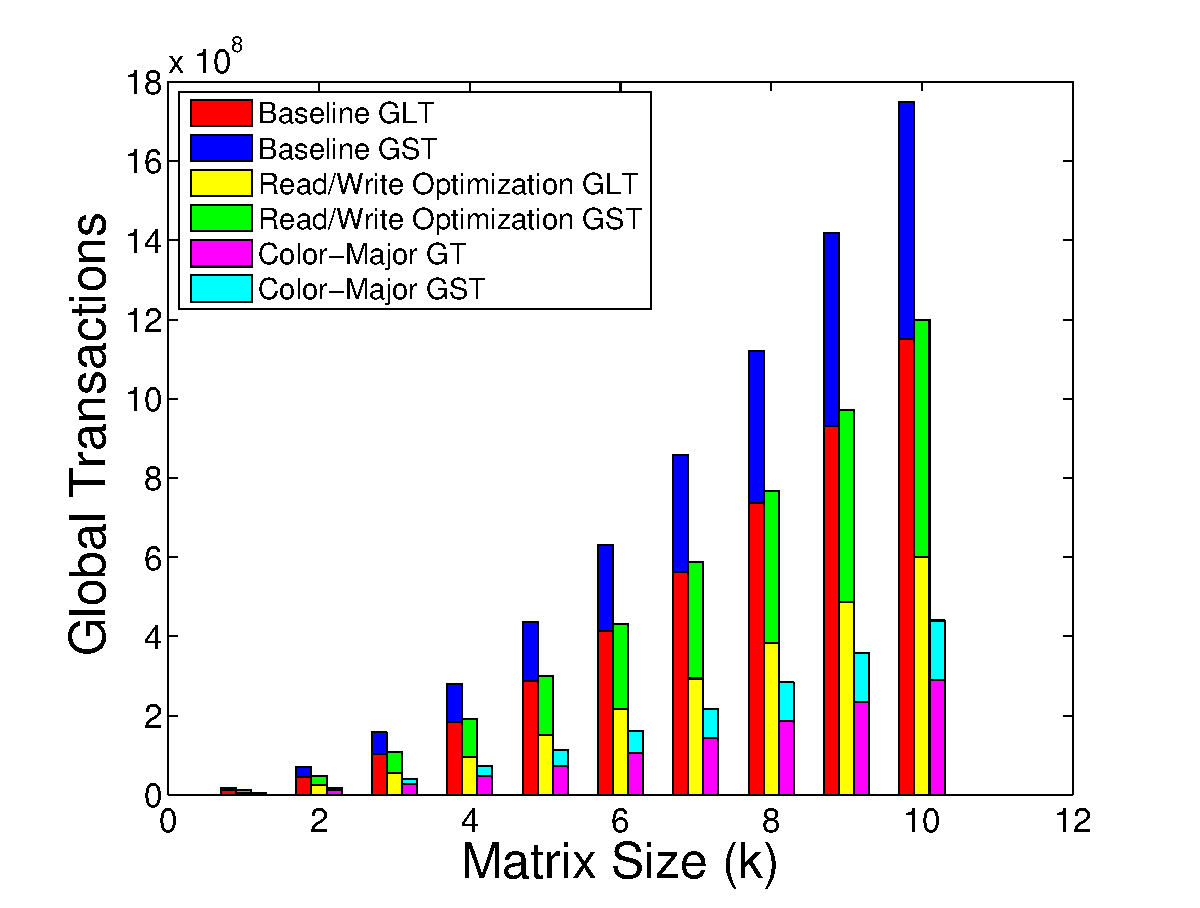
\includegraphics[width=0.5\textwidth]{transaction}
%\caption{Transactions on Singular Vector Design. \textcolor{blue}{GLT represents Global Load Transaction. GST presents Global Store Transaction}}
%\label{fig:transaction}
%\end{figure}
%%\begin{figure}[hbpt]
%%\centering
%%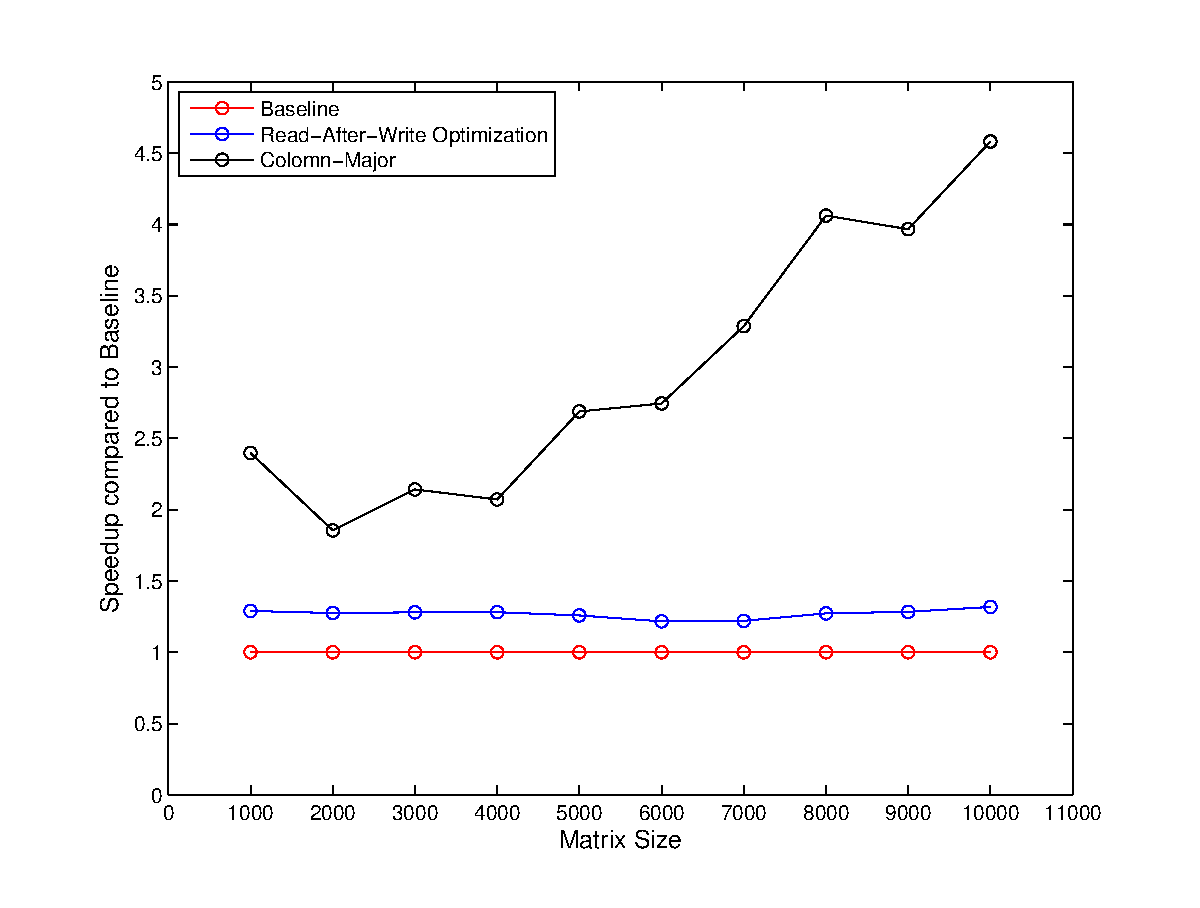
\includegraphics[width=0.5\textwidth]{vector_kernels}
%%\caption{Transactions on Singular Vector Design}
%%\label{fig:vector_kernels}
%%\end{figure}
%Read transactions are about twice of the write transactions on the global memory.
%Further analysis reveals that about 50\% of global memory transfers are read-after-write.
%Since it is a waste of time to read from global memory after writing to global memory,
%we improve the memory access performance by copying these values into the local memory and shared memory of the GPU.
%The global read transactions are reduced by 50\% compared to the baseline, while the write transactions remain the same, as shown as ``read/write optimization'' in Figure \ref{fig:transaction}. The speedup reaches to 1.2X compared to the baseline.
%To further optimize the access to the global memory,
%we change the matrix arrangement from row-major to column-major in the global memory. 
%As a result, the global load/store transactions are reduced by 50\%/25\% compared to ``read/write optimization'', respectively. 
%This is because column-major matrix have coalesced global memory accesses, which saves hundreds of transactions per thread. The speedup rises up to 4.5X compared to the baseline.

\subsection{Solution to Huge Matrices}
\label{sec_huge}
In our design, the maximum number of singular values can be processed on a singular GPU is $m_b = subinterval\_size \times thread\_block\_size$,
while the maximum number of singular vectors are determined by Equation (\ref{eq:max_size}).
\begin{equation}
m_t = \sqrt{U / (5 * S)}
\label{eq:max_size}
\end{equation}
where $U$ is the memory size of GPU, $5$ is the number of arrays required for a pair of singular vectors.
Usually, $m_b$ is much larger than $m_t$.
For Tesla K40c with 16GB memory, $m_t = 24K$, while $m_b = 262K$.
However, when the matrix size is larger than $m_t$, even larger than $m_b$,
the GPU kernels cannot obtain all singular values and vectors any more with a single GPU.
Therefore we derive a divide-and-conquer architecture to solve the huge matrix size as explained in this section.

When the size of a matrix is less than $m_b$ but larger than $m_t$,
we only need to divide the singular vectors into small sets, each of which can be processed by a single GPU.
However, if the matrix size is larger than $m_b$, we should divide both singular values and singular vectors into smaller partitions.
The singular value computations can be partitioned using $m_b$ directly, i.e., there are $l_b = \lfloor(n/m_b)\rfloor + 1$ partitions, each of which has $\lfloor(n/l_b)\rfloor$ singular values.

The division of singular vectors should take memory size into consideration.
The maximum number of partitions $l_t$ can be derived from Equation~(\ref{eq:max_length}) as follows:
\begin{equation}
l_t = \sqrt{U/(5 * n * 4)}
\label{eq:max_length}
\end{equation}
where $n$ is matrix size.
Thus, there should be $\lfloor(n/l_t)\rfloor+1$ partitions with
$\lfloor(n/l_t)\rfloor$ singular vectors in each partition.

% \subsubsection{Single GPU}
% For a single GPU, the execution between every pieces is serial {\bf FIXME: need discussion}.
% When one piece is finished, the GPU processes the next one, until the last one.
% Thus, the execution time is the summation of every data segment.
% Equation \ref{eq:max_length} also provides the theorical maximum matrix size can be processed on GPUs when set $l=1$.
% For Tesla K40c, the theorical maximum matrix size is $600$ million.
% However, only one thread works on GPU, if $l=1$.
% The singular vector kernel will not have any speedup compared to execution on CPU. {\bf FIXME this seems to be a big drawback of the design. We have to address this}

\subsection{Multiple GPUs on a server}
\label{sec_mgpu}
We implement the multiple-GPU version with Pthread libraries on one server
to control data partition and assignment to GPUs.
Pthreads is a nature choice for controlling multiple GPUs on a single server
because it uses shared memory architecture, dramatically reducing overheads
on data sharing. We also design an extensible interface between CPU and GPU,
 which is easy to scale to physical distributed GPUs, compared to CUDA asynchronization interface. In our design, each thread takes control of one GPU.

%According to the computing capacity of GPU, we separate the whole interval into several subintervals with different singular values in them.
%Each GPU processes its corresponding subintervals to obtain singular values and vectors.
%\textcolor{red}{Is this correct? is it "Each thread processes its corresponding subinterval to obtain singular values and vectors."?}

When matrix size becomes huge, the load balancing among multiple GPUs will be a problem for performance as shown in column 2 of Table \ref{tab:hugeResultTesla}.
To conquer this issue we also introduce a dynamic load-balancing method for a better speedup, where a GPU will take new tasks on unfinished subintervals as soon as it finishes its prior task.
%In this method, the whole intervals are divided into small pieces which can be processed in one GPU.
%when one GPU finishes its tasks and other GPU, it will check the tasks of other GPUs.

%\textbf{algorithm graph}
%For each subinterval, there are four global state : FREE, READY, BUSY, DONE.
%FREE means that the singular values in the subinterval have not been calculated yet.
%READY represents that singular value is ready to wait for further processing singular vector.
%BUSY is in the precessing of singular vectors.
%DONE means the singular vectors are ready in the subintervals.
%When singular values are READY, GPU will continue to calculate the singular vectors and set the state to BUSY.


%We also build a two-computer network to speed up the SVD.
%In our design, each computer has one GPU and communicated through sockets.

